\section{Parser}
\begin{frame}
\tableofcontents[currentsection]
\end{frame}
\subsection{Socket}
\subsection{Einleitung}

\frame
{
  \frametitle{Einleitung}
  \begin{itemize}
    \item NAO wird in einem Simulator ausgef\"uhrt
  \end{itemize}
  \begin{center}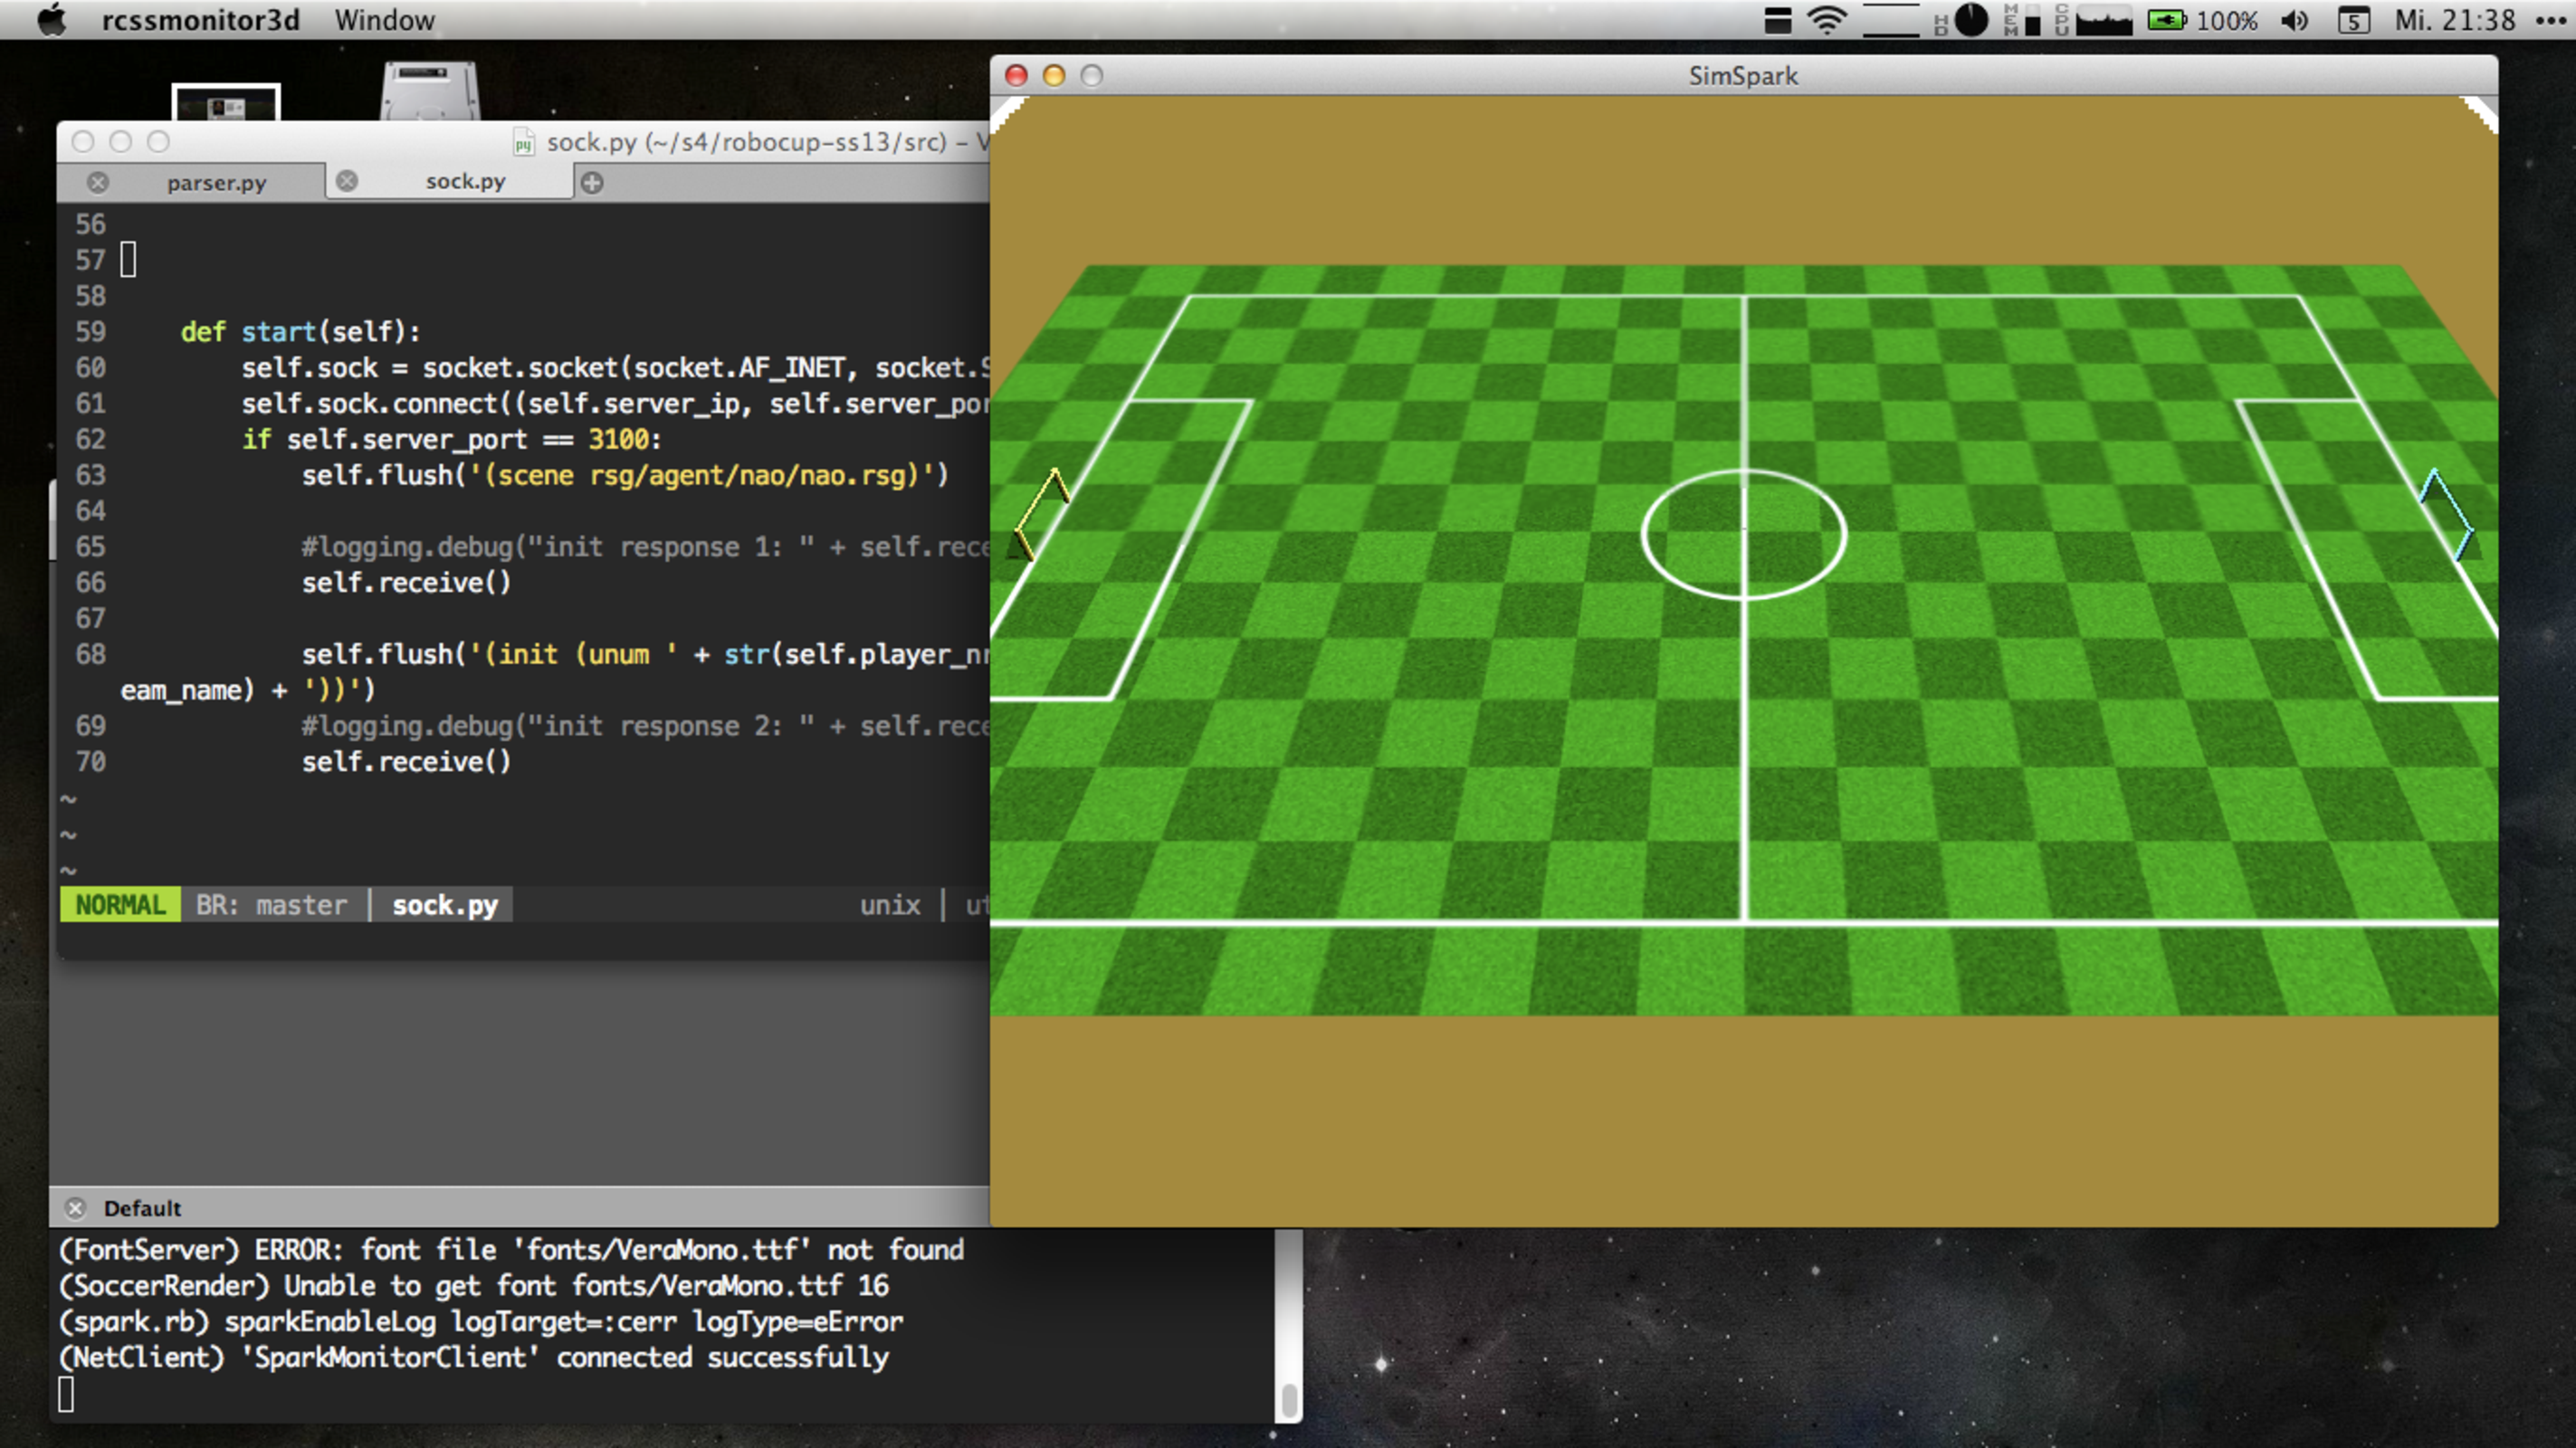
\includegraphics[height=5cm, center]{simulator.pdf}\end{center}
}
  
\frame
{
  \frametitle{Einleitung}
  \begin{itemize}
    \item Die Erkennung der Sensoren des NAO ist eingebaut.
    \item Wir verbinden uns via Socket zum NAO
  \end{itemize}
  
  \begin{center}\tiny{Server: \ttfamily{localhost}\\ Port: \ttfamily{3100}}\end{center}
}

\frame
{
  \frametitle{Einleitung}
  \begin{itemize}
    \item Der NAO sendet Sensordaten und empf\"angt Befehle als S-Expression:\\\vskip0.5cm
  \tiny{\ttfamily{(See
  (G2R (pol 17.55 -3.33 4.31))
  (G1R (pol 17.52 3.27 4.07))
  (F1R (pol 18.52 18.94 1.54))
  (F2R (pol 18.52 -18.91 1.52))
  (B (pol 8.51 -0.21 -0.17))
  (P  (team teamRed) (id 1)
      (head (pol 16.98 -0.21 3.19))
      (rlowerarm (pol 16.83 -0.06 2.80))
      (rfoot (pol 17.00 0.29 1.68))
  )
  (L (pol 12.97 -37.56 -2.24)
     (pol 13.32 -32.98 -2.20))
)}}\end{itemize}\begin{itemize}
    \item Wie nutzen wir diese Daten?
  \end{itemize}
}

\subsection{Parser}
\frame
{
  \frametitle{Parser}
  
  \begin{itemize}[<+->]
    \item Endlosschleife wartet auf Empfang neuer Daten
    \item Ein regul\"arer Ausdruck zergliedert rekursiv die S-Expression\\
    \lstinputlisting{regexp.txt}
    \item Die entstandene Liste wird anschlie{\ss}end ins Weltmodell des NAO eingepflegt
  \end{itemize}
}

\subsection{Probleme}
\frame
{
  \frametitle{Probleme}
  
  \begin{itemize}
    \item Fehler im Regul\"aren Ausdruck, Parameter der Sensoren wurden nicht erkannt
  \end{itemize}
}
